

\chapter{Resultados}
\thispagestyle{fancy}
\label{ch:resultados}

\section{Datos en Bruto}

A continuación, se presentan las tablas con los datos en bruto obtenidos durante el proceso de medición para cada uno de los sólidos estudiados: el cilindro de corcho, el cilindro plateado, el cilindro dorado, el cilindro hueco y la moneda. Estos datos incluyen las mediciones directas de masa, longitud y diámetro realizadas con los instrumentos correspondientes, así como las repeticiones necesarias para obtener un valor promedio representativo.
% --- Tabla: Corcho ---
\begin{table}[h!]
    \centering
    \caption{Mediciones directas para el cilindro de corcho.}
    \label{tab:corcho}
    \begin{tabular}{ccc}
    \toprule
    \textbf{Largo (cm)} & \textbf{Diámetro (cm)} & \textbf{Masa (g)} \\
    \midrule
    3.745 & 1.400 & 3.22 \\
    3.745 & 1.435 & 3.22 \\
    3.750 & 1.400 & 3.22 \\
    3.750 & 1.435 & 3.22 \\
    3.750 & 1.430 & 3.22 \\
    3.800 & 1.435 & 3.22 \\
    3.800 & 1.440 & 3.22 \\
    3.800 & 1.430 & 3.22 \\
    3.800 & 1.430 & 3.22 \\
    3.750 & 1.435 & 3.22 \\
    3.800 & 1.435 & 3.22 \\
    3.740 & 1.435 & 3.22 \\
    \bottomrule
    \end{tabular}
\end{table}

% --- Tabla: Cilindro Plateado ---
\begin{table}[h!]
    \centering
    \caption{Mediciones directas para el cilindro plateado.}
    \label{tab:cilindro_plata}
    \begin{tabular}{ccc}
    \toprule
    \textbf{Largo (cm)} & \textbf{Diámetro (cm)} & \textbf{Masa (g)} \\
    \midrule
    1.620 & 1.100 & 17.84 \\
    1.620 & 1.100 & 17.84 \\
    1.620 & 1.100 & 17.84 \\
    1.620 & 1.100 & 17.84 \\
    1.620 & 1.100 & 17.84 \\
    1.620 & 1.100 & 17.84 \\
    1.620 & 1.100 & 17.84 \\
    1.620 & 1.100 & 17.84 \\
    1.620 & 1.100 & 17.84 \\
    1.620 & 1.100 & 17.84 \\
    1.620 & 1.100 & 17.84 \\
    1.615 & 1.100 & 17.84 \\
    \bottomrule
    \end{tabular}
\end{table}

% --- Tabla: Cilindro Dorado ---
\begin{table}[h!]
    \centering
    \caption{Mediciones directas para el cilindro dorado.}
    \label{tab:cilindro_dorado}
    \begin{tabular}{ccc}
    \toprule
    \textbf{Largo (cm)} & \textbf{Diámetro (cm)} & \textbf{Masa (g)} \\
    \midrule
    1.660 & 1.100 & 43.78 \\
    1.660 & 1.100 & 43.78 \\
    1.655 & 1.100 & 43.78 \\
    1.660 & 1.100 & 43.78 \\
    1.655 & 1.100 & 43.78 \\
    1.660 & 1.100 & 43.78 \\
    1.655 & 1.100 & 43.78 \\
    1.660 & 1.100 & 43.78 \\
    1.665 & 1.100 & 43.78 \\
    1.665 & 1.100 & 43.78 \\
    \bottomrule
    \end{tabular}
\end{table}

% --- Tabla: Cilindro Hueco ---
\begin{table}[h!]
    \centering
    \caption{Mediciones directas para el cilindro hueco.}
    \label{tab:cilindro_hueco}
    \begin{tabular}{cccc}
    \toprule
    \textbf{Largo (cm)} & \textbf{D. Externo (cm)} & \textbf{D. Interno (cm)} & \textbf{Masa (g)} \\
    \midrule
    1.565 & 1.100 & 0.840 & 3.26 \\
    1.570 & 1.100 & 0.885 & 3.26 \\
    1.565 & 1.100 & 0.885 & 3.26 \\
    1.570 & 1.100 & 0.885 & 3.26 \\
    1.565 & 1.100 & 0.875 & 3.26 \\
    1.565 & 1.100 & 0.870 & 3.26 \\
    1.565 & 1.100 & 0.875 & 3.26 \\
    1.565 & 1.100 & 0.875 & 3.26 \\
    1.565 & 1.100 & 0.875 & 3.26 \\
    1.565 & 1.100 & 0.875 & 3.26 \\
    \bottomrule
    \end{tabular}
\end{table}

% --- Tabla: Moneda ---
\begin{table}[h!]
    \centering
    \caption{Mediciones directas para la moneda.}
    \label{tab:moneda}
    \begin{tabular}{ccc}
    \toprule
    \textbf{Espesor (cm)} & \textbf{Diámetro (cm)} & \textbf{Masa (g)} \\
    \midrule
    0.137 & 3.910 & 9.50 \\
    0.135 & 3.910 & 9.50 \\
    0.138 & 3.910 & 9.50 \\
    0.135 & 3.910 & 9.50 \\
    0.135 & 4.005 & 9.50 \\
    0.135 & 4.005 & 9.50 \\
    0.133 & 4.005 & 9.50 \\
    0.138 & 3.910 & 9.50 \\
    0.135 & 4.005 & 9.50 \\
    0.137 & 3.910 & 9.50 \\
    0.133 & 4.005 & 9.50 \\
    0.137 & 4.005 & 9.50 \\
    \bottomrule
    \end{tabular}
\end{table}

\clearpage

\section{Cálculos y Discusión}

Se realizó el proceso de análisis de datos para cada sólido
utilizando las mediciones directas obtenidas en la sección anterior.
 Para cada sólido, se calcularon las magnitudes indirectas de volumen y densidad,
 a partir de las siguientes fórmulas geométricas:
\begin{itemize}
    \item $V = \pi r^{2} h$ para los cilindros.
    \item  $V = \pi h (R^{2} - r^{2})$ para el cilindro hueco, donde $R$ es el radio externo y $r$ el radio interno.
    \item $\rho = \frac{m}{V}$
\end{itemize}

El error  propagado fue estimado  utilizando la suma lineal de las derivadas parciales 
multiplicadas por las incertidumbres absolutas de cada variable, 
siguiendo el criterio del peor escenario.

% --- Resultados Volumen ---
\begin{table}[h!]
\centering
\caption{Resultados de Volumen y Error Relativo}
\label{tab:masa_vol}
    \begin{tabular}{lccc}
    \toprule
    Objeto & Volumen ($cm^3$) & $E_V$ (\%) \\
    \midrule
    Corcho & $6.039 \pm 0.050$ & 0.83\% \\
    Cilindro Plateado & $1.539 \pm 0.019$ & 1.23\% \\
    Cilindro Dorado & $1.577 \pm 0.019$ & 1.20\% \\
    Cilindro Hueco & $0.549 \pm 0.026$ & 4.74\% \\
    Moneda & $1.669 \pm 0.017$ & 1.02\% \\
    \bottomrule
    \end{tabular}
\end{table}

\vspace{0.5cm} % Espacio entre tablas

Se observa que el cilindro hueco presenta el mayor error relativo en el 
volumen, esto se debe a que la incertidumbre en el diámetro interno 
tiene un impacto significativo en el cálculo del volume, pues le añade 
una fuente adicional de error. En contraste, el corcho, a pesar de ser un 
sólido irregular, muestra un error relativo menor a los cilindros regulares, 
curiosamente este fue el sólido que tuvo más repeticiones en las mediciones para 
contrarrestar su irrregularidad, además de más cálculos de masa por diferencia; 
lo que marca un indicio a que los cilindros regulares pueden presentar
errores sistemáticos por la técnica de medición, así como también errores
aleatorios por la variabilidad en la posición del instrumento.
Luego del corcho, se observa que la moneda presenta el segundo menor error 
relativo en volumen, esto se debe a que su forma es más regular y 
las mediciones de diámetro y espesor fueron realizadas con
instrumentos de mayor precisión (micrómetro para el espesor),
lo que contribuyó a reducir la incertidumbre en el cálculo del volumen.
Aquí, se puede inferir que la apreciación del vernier puede no ser 
suficiente para medir con precisión los cilindros, lo que sugiere que 
el uso de un micrómetro para estas mediciones sería más adecuado 
para reducir el error relativo en el volumen, y en consecuencia, en la densidad.

Adicionalmente, se observó que los cilindros, especialmente la parte interior 
del cilindro hueco, presentaban desniveles y pequeñas irregularidades en la 
superficie.
Estos desgastes y pequeñas deformaciones pueden haber contribuido al aumento 
de la incertidumbre en las mediciones; podían ser vistos al detallar la
superficie a la luz.

% --- Resultados de Densidad y Error Relativo ---
\begin{table}[h!]
\centering
\caption{Resultados de Densidad y Error Relativo}
\label{tab:densidad}
    \begin{tabular}{lcc}
    \toprule
    Objeto & Densidad ($g/cm^3$) & $E_{\rho}$ (\%) \\
    \midrule
    Corcho & $0.53 \pm 0.01$ & 1.89\% \\
    Cilindro Plateado & $11.59 \pm 0.15$ & 1.29\% \\
    Cilindro Dorado & $27.76 \pm 0.34$ & 1.22\% \\
    Cilindro Hueco & $5.94 \pm 0.30$ & 5.05\% \\
    Moneda & $5.69 \pm 0.06$ & 1.05\% \\
    \bottomrule
    \end{tabular}
\end{table}

Notablemente el cilindro dorado posee una densidad sospechosamente alta,
esto sugiere que la balanza granataria pudo haber presentado un 
error sistemático, ya que incluso es mayor que la densidad del Osmio,
el metal natural más denso conocido, lo que es físicamente imposible para un sólido común.
Este error sistemático también se podría ver reflejado en el corcho, 
que a pesar de haber sido el sólido con menor error relativo en volumen,
presenta un error relativo en densidad mayor que el cilindro plateado, 
lo que sugiere que la medición de masa pudo haber sido afectada por este mismo error.

Adicionalmente, se puede destacar que el corcho tiene una densidad mayor 
al promedio comercial, lo que podría deberse a este mismo error en la balanza, o
incluso que el corcho utilizado en la práctica tenía más humedad de lo esperado.

\begin{figure}[h!]
    \centering
    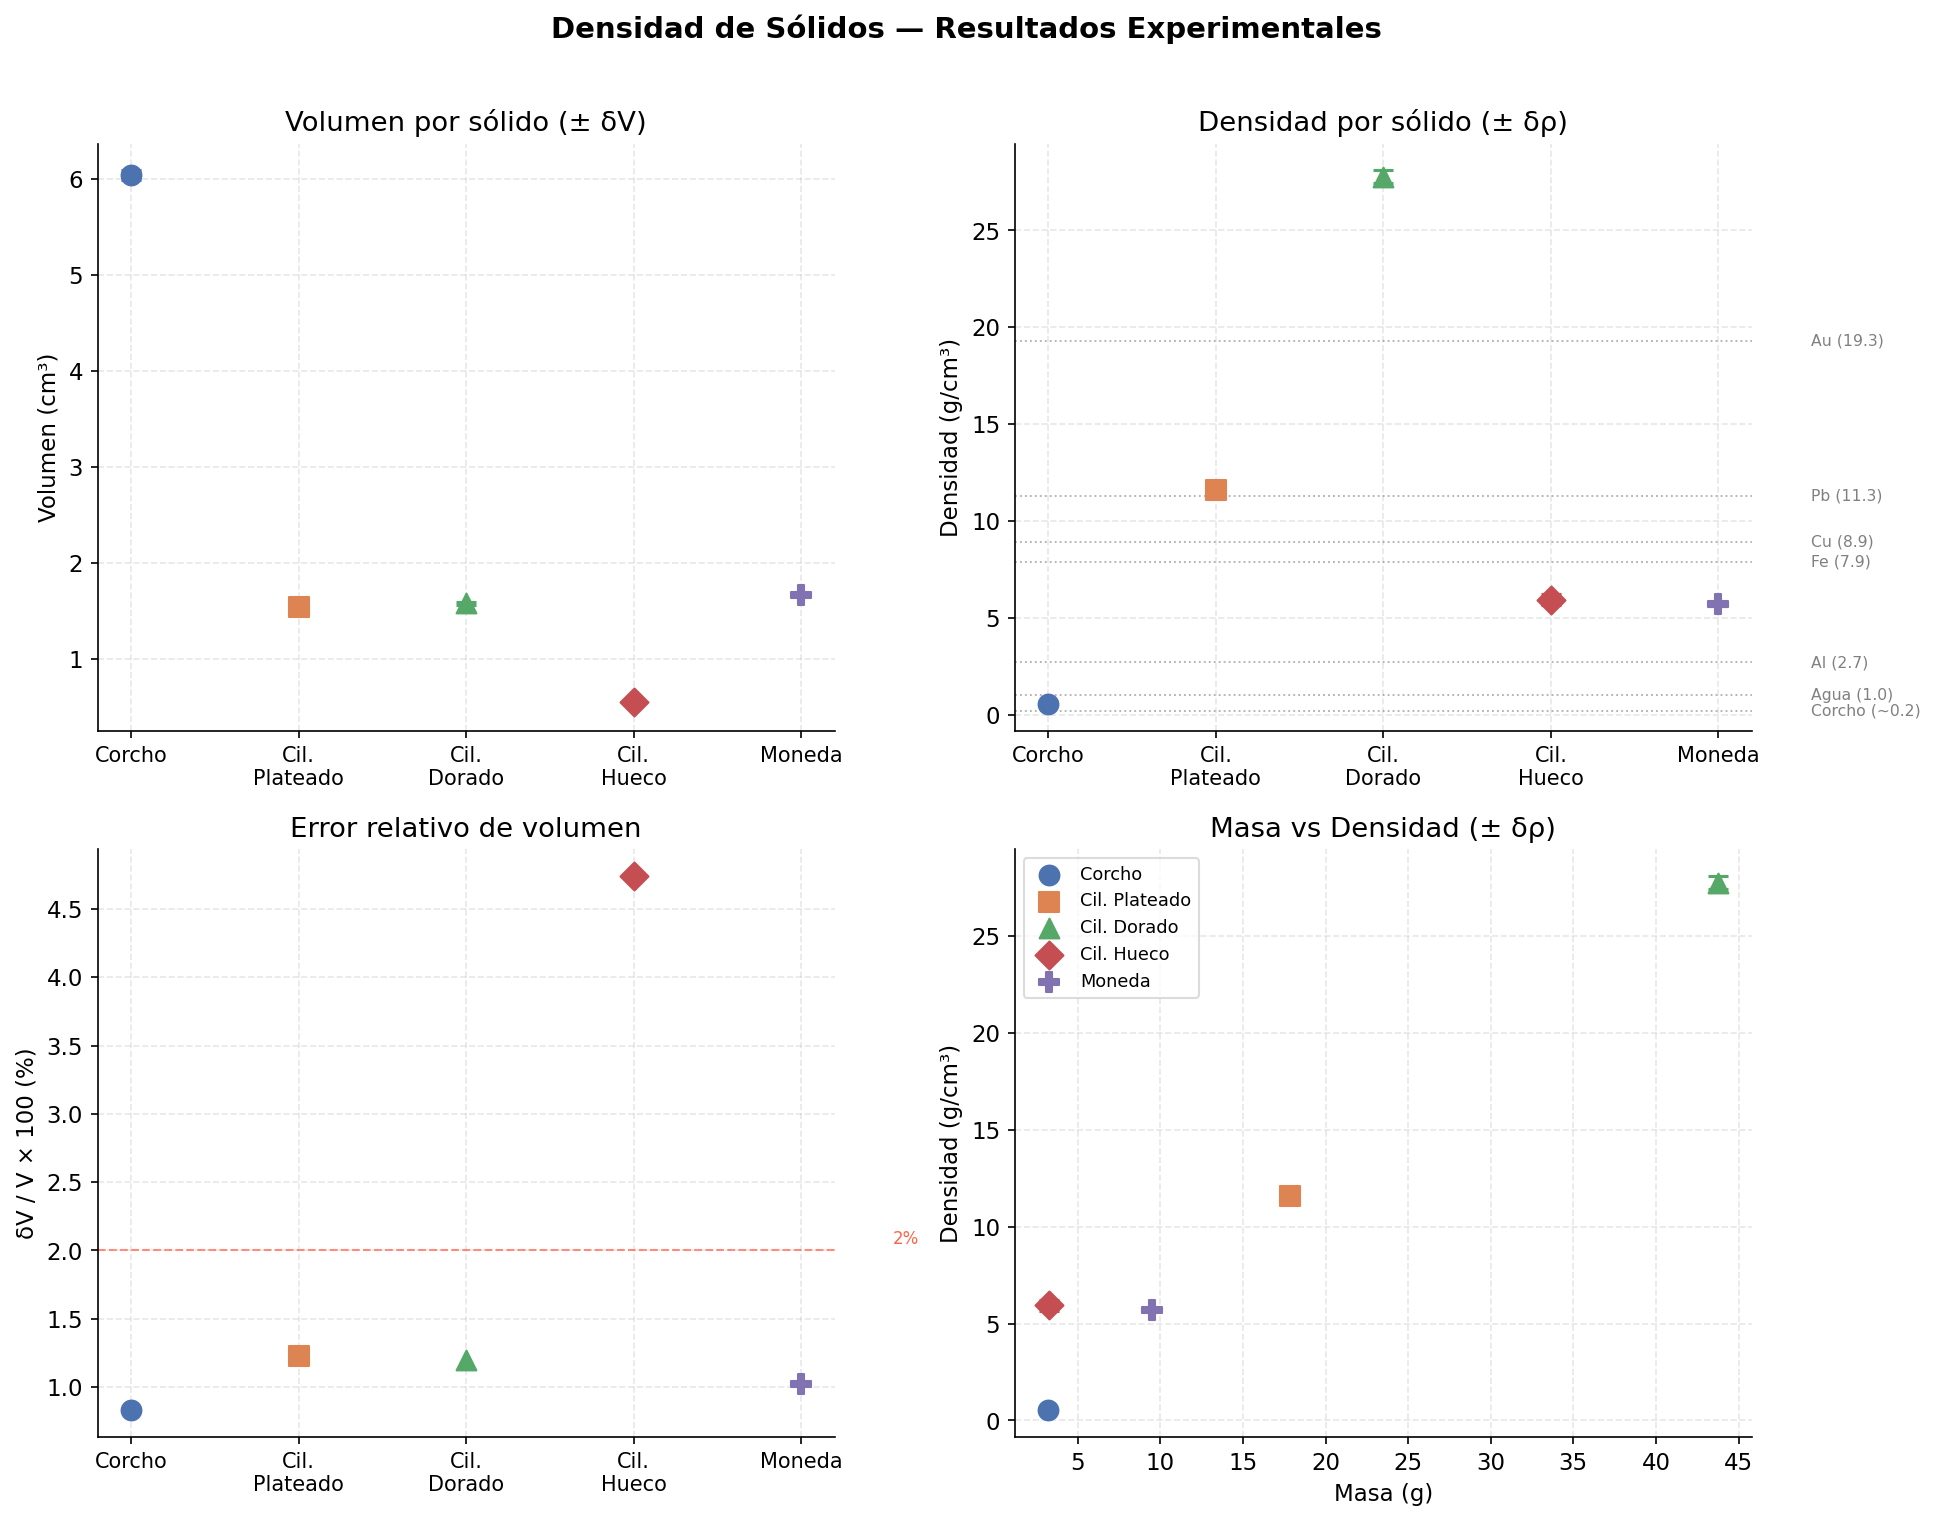
\includegraphics[width=1\textwidth]{imagenes/graficas_laboratorio.png}
    \caption{Gráfica sobre los resultados indirectos}
    \label{fig:grafica}
\end{figure}

 